\documentclass{article}

% if you need to pass options to natbib, use, e.g.:
% \PassOptionsToPackage{numbers, compress}{natbib}
% before loading rl_project.

% to compile a camera-ready version, add the [final] option, e.g.:
 \usepackage[final]{rl_project}

% to avoid loading the natbib package, add option nonatbib:
% \usepackage[nonatbib]{rl_project}

\usepackage[utf8]{inputenc} % allow utf-8 input
\usepackage[T1]{fontenc}    % use 8-bit T1 fonts
\usepackage{hyperref}       % hyperlinks
\usepackage{url}            % simple URL typesetting
\usepackage{booktabs}       % professional-quality tables
\usepackage{amsfonts}       % blackboard math symbols
\usepackage{nicefrac}       % compact symbols for 1/2, etc.
\usepackage{microtype}      % microtypography
\usepackage{graphicx}
\usepackage{tikz}
\usepackage{float}
\usepackage{amsmath}
\usetikzlibrary{arrows.meta, positioning}

% Give your project report an appropriate title!

\title{RL Project Template}
% Your report should be written using the provided LaTeX template, and should be no longer than seven pages including figures but excluding references and appendices. The content of all figures, including any embedded text, should be clearly legible; you will lose marks for figures and text that are too small to view comfortably. You should not modify the provided LaTeX template. Any appendices should be clearly referenced in the main body of your report. All sources should be referenced appropriately. Each group should submit a single report. This coursework is not marked anonymously.

% The \author macro works with any number of authors. There are two
% commands used to separate the names and addresses of multiple
% authors: \And and \AND.
%
% Using \And between authors leaves it to LaTeX to determine where to
% break the lines. Using \AND forces a line break at that point. So,
% if LaTeX puts 3 of 4 authors names on the first line, and the last
% on the second line, try using \AND instead of \And before the third
% author name.

\author{
  David Hood, Vanisha Oree, Loving-Grace Mawire
  \\
  Department of Computer Science\\
  University of Bath\\
  Bath, BA2 7AY \\
  \texttt{dh2155@bath.ac.uk} \\
  \texttt{vo256@bath.ac.uk} \\
  \texttt{lgrm21@bath.ac.uk}\\
  %% examples of more authors
  %% \And
  %% Coauthor \\
  %% Affiliation \\
  %% Address \\
  %% \texttt{email} \\
  %% \AND
  %% Coauthor \\
  %% Affiliation \\
  %% Address \\
  %% \texttt{email} \\
  %% \And
  %% Coauthor \\
  %% Affiliation \\
  %% Address \\
  %% \texttt{email} \\
  %% \And
  %% Coauthor \\
  %% Affiliation \\
  %% Address \\
  %% \texttt{email} \\
}

\begin{document}

\maketitle

\section{Problem Definition}
% A clear, precise and concise description of your chosen problem, including the states, actions, transition dynamics, and the reward function. You will lose marks for an unclear, incorrect, or incomplete problem definition. You should also discuss the difficulty of your chosen problem and justify why it cannot be solved effectively using tabular reinforcement learning methods.
Our chosen problem is learning to play the Atari game \textbf{Pong} using reinforcement learning. Pong is a two-player zero sum game where each player controls a vertical paddle and attempts to return a moving ball past the opponent. A point gets scored when the opponent fails to return the ball. The aim of the agent is to maximize the cumulative reward over an episode by learning how to control the paddle optimally.

This problem is formulated as a \textbf{Markov Decision Process} defined by the tuple \((\mathcal{S}, \mathcal{A}, \mathcal{P}, \mathcal{R}, \gamma)\), where where \(\mathcal{S}\) is the state space, \(\mathcal{A}\) is the action space, \(\mathcal{P}\) is the transition dynamics, \(\mathcal{R}\) is the reward function, and \(\gamma\) is the discount factor.
% overview of state space, action and transition dynamics 
\subsection{State Space}
The state at time step \(t\), denoted \(s_t \in \mathcal{S}\), is constructed from the last four consecutive preprocessed game frames. Each frame is:

\begin{itemize}
    \item Converted to \textbf{grayscale}
    \item Resized to \textbf{84 $\times$ 84 pixels}
    \item Normalised to values in \([0,1]\)
\end{itemize}

Thus, we can represent the state as:
\[
s_t = (x_{t-3}, x_{t-2}, x_{t-1}, x_t)
\]
where each \(x_t \in \mathbb{R}^{84 \times 84}\). 
The full state therefore has shape \textbf{(84, 84, 4)}.
% explain the four frames stacking
The concept behind stacking four frames is to provide the agent with \textbf{temporal information}, allowing it to infer ball velocity and direction, which cannot be determined from a single static frame. 

\subsection{Action Space}
The action space \(\mathcal{A}\) is discrete and consists of the legal paddle movements available to the agent in Pong. These six actions in this game are:

\begin{itemize}
    \item No operation (do nothing)
    \item Move paddle up
    \item Move paddle down
    \item Fire
    \item Paddle up + Fire
    \item Paddle down + Fire
\end{itemize}

At each time step, the agent selects one action \(a_t \in \mathcal{A}\), which is applied for several internal frames due to frame skipping.

\subsection{Transition Dynamics}
The transition dynamics \(\mathcal{P}(s_{t+1} | s_t, a_t)\) are governed by the \textbf{deterministic physics of the Atari game engine} combined with the opponent’s policy. The agent does not control the opponent paddle, which behaves according to a built-in strategy.

Due to unknown opponent behaviour, partial observability from individual frames, and frame skipping, the exact transition probabilities are unknown and cannot be modelled explicitly.

\subsection{Reward Function}
The reward function \(\mathcal{R}(s_t, a_t)\) is defined as:
\begin{itemize}
    \item \textbf{+1} when the agent scores a point
    \item  \textbf{-1} when the opponent scores a point
    \item \textbf{0} otherwise
\end{itemize}

An episode ends when one player reaches a terminal score. 
The goal of the agent is to maximize the total reward (per episode), which corresponds to winning the match. 

\subsection{Problem Difficulty}
Pong is a high-dimensional, continuous visual control task with the following challenges:

\begin{enumerate}
    \item High Dimensional State Space: Each state consists of over 28,000 pixels (84 $\times$ 84 $\times$ 4).
    \item Observability: A single frame does not have information about motion (although a stacked set of frames does convey motion).
    \item Non-Stationarity: The opponent and ball dynamics are continuously changing.
    \item Delayed rewards: Learning is difficult given actions that                           influence success or failure receive feedback many steps later, preventing          the agent from associating individual actions with their outcomes.
    \item Ambiguous feedback: Actions taken early in a Pong rally affect the outcome          much later, requiring the agent to correctly attribute sparse and delayed           rewards to distant decisions.
\end{enumerate}

\subsection{Why Tabular Reinforcement Learning is not feasible}

Tabular reinforcement learning methods such as standard Q-learning require storing a value for every state--action pair. However, in Pong, the state space derived from raw pixel observations is both continuous and extremely high dimensional. Each frame contains thousands of pixel values, and the agent must also infer motion from multiple consecutive frames. Attempting to treat each possible pixel configuration as a distinct state would be infeasible. Even if the image were discretised coarsely, the number of resulting state configurations would still be astronomically large.

Furthermore, successful control requires the agent to generalise across visually similar states (for example, slightly different ball positions or paddle offsets) rather than storing separate values for every possible configuration. Tabular reinforcement learning methods cannot provide this generalisation and would require a Q-table far too large to construct or learn efficiently.

To overcome these limitations, the agent must use a function approximator that can map high-dimensional visual inputs to action values. A Deep Q-Network (DQN) based on convolutional neural networks is therefore employed to approximate the optimal action-value function:
\[
Q(s, a; \theta)
\]
This approach enables learning directly from raw pixels by exploiting spatial and temporal regularities in the observations, allowing the agent to scale to the large state space.


\section{Background}
% A discussion of reinforcement learning methods that may be effective at solving your chosen problem, their strengths and weaknesses for your chosen problem, and any existing results in the scientific literature (or publicly available online) on your chosen problem or similar problems. (LGM)

\subsection{Foundations of Reinforcement Learning}
Reinforcement Learning (RL) is a framework in which agents learn to make decisions through interaction with an environment. The agent observes its current situation, selects an action, receives a reward, and transitions to a new situation. Over time, it learns to maximise the cumulative reward it receives. Most RL problems are formalised using the framework of a Markov Decision Process (MDP) (Sutton and Barto, 2018). An MDP defines the environment in terms of a set of states, a set of available actions, a reward function, a transition function, and a discount factor. The Markov property assumes that the next state and reward depend only on the current state and action, not on the full history of past interactions.

In RL, the agent’s goal is to learn a policy, a mapping from states to actions, that maximises expected long-term reward. 

\subsection{Types of Reinforcement Learning Methods}
There are several classes of RL algorithms. Model-free methods learn from experience without building an explicit model of the environment's dynamics. In contrast, model-based methods aim to learn a predictive model of the environment, which can be used for planning and decision-making (Huang, 2020).

Within the model-free category, two major subtypes are value-based and policy-based methods. Value-based methods focus on estimating the value of taking a particular action in a particular state. One of the best-known examples is Q-learning, where the agent learns an action-value function that approximates the expected return for each state-action pair. Policy-based methods, on the other hand, aim to learn the policy directly. These approaches are particularly effective in continuous action spaces or where stochastic policies are beneficial. However, they often exhibit higher variance and can require careful tuning of hyperparameters (Greensmith et al., 2004). 

Policy gradient methods, such as REINFORCE or Proximal Policy Optimisation (PPO), directly optimise the policy rather than estimating value functions. These methods are advantageous in environments with continuous or high-dimensional action spaces and can represent stochastic policies. However, they are generally more sensitive to hyperparameter choices and can suffer from high variance in the gradient estimates. While PPO includes mechanisms to reduce this variance, it still requires careful tuning and may be less efficient in environments with discrete actions such as Pong (Papini et al., 2018).

Model-based reinforcement learning is another alternative. These methods attempt to learn a model of the environment's dynamics, which can be used to simulate experiences and improve sample efficiency. In theory, model-based methods require fewer real interactions with the environment. However, learning accurate models from high-dimensional visual data is extremely challenging (Moerland et al., 2020). In practice, errors in the learned model can lead to poor generalisation and suboptimal behaviour. Recent work in world models and latent-space planning has made progress, but model-free approaches such as DQN remain more robust and reliable in visual domains like Pong (Ha and Schmidhuber, 2018).

\subsection{Deep Q-Learning and Visual Environments}
Q-learning in its tabular form performs well in small environments with discrete, low-dimensional state spaces. However, in environments with large or continuous state spaces, such as those involving visual inputs from games, it becomes infeasible to maintain a Q-table (Adhikari and Ren, 2021). This limitation led to the development of function-approximated methods, particularly those using deep neural networks.

The Deep Q-Network (DQN) algorithm (Mnih et al., 2015) represents a significant advance in this area. DQN approximates the Q-value function using a convolutional neural network (CNN), allowing it to learn directly from raw pixel input. This made it possible to apply reinforcement learning successfully to high-dimensional, visual domains such as Atari games. The agent receives a stack of consecutive frames as input and outputs a Q-value for each possible action. Over time, it learns to associate visual patterns with successful strategies.

To stabilise training, DQN introduces two core innovations. The first is experience replay, which stores past transitions and samples them randomly during training. This reduces the correlation between training samples and improves sample efficiency. The second is the use of a target network, which is updated less frequently than the main network. This helps to reduce instability by decoupling the network used to estimate the Q-value target from the one being updated.

\subsection{Application to Pong and Relevant Enhancements}
DQN is particularly well-suited to our problem, which involves learning to play the game Pong from pixel inputs. Pong presents a challenging environment with sparse rewards, temporal dependencies, and a discrete action space. DQN has been shown to perform well in such conditions, achieving superhuman performance in the original DeepMind experiments (Mnih et al., 2015). The convolutional architecture is well-matched to the image-based state representation, while the use of experience replay allows the agent to learn efficiently from limited reward signals.

Despite its strengths, DQN is not without limitations. It has been shown to suffer from overestimation bias, where Q-values are systematically overestimated due to the use of the max operator in the Bellman update. To address this, Double DQN was proposed, which separates the selection and evaluation of actions to reduce this bias (Hasselt, Guez and Silver, 2016). Another improvement is Dueling DQN, which decomposes the Q-value into two streams: one estimating the value of being in a state, and the other estimating the advantage of each action. This helps the agent learn more efficiently in environments where many actions have similar outcomes. Additionally, Prioritised Experience Replay has been introduced to sample more informative transitions more frequently, improving convergence speed (Schaul et al., 2016; Huang, Wei and Wang, 2018).

While these extensions offer measurable improvements, our project focuses on implementing and analysing the baseline DQN algorithm. The decision to use DQN is motivated by its proven success in learning from pixels in environments with discrete actions and sparse rewards. The game Pong has become a standard benchmark in the Arcade Learning Environment (ALE) and continues to be widely used in academic and applied research to evaluate reinforcement learning algorithms. Numerous replications and open-source implementations of DQN have demonstrated its effectiveness in this domain.


\section{Method}
% A description of the method(s) used to solve your chosen problem, an explanation of how these methods work (in your own words), and an explanation of why you chose these specific methods.
 % process workflow: Appendix A - Figure 2

We use the Deep Q-Network (DQN) algorithm to train an agent to play Atari Pong directly from sequences of pixel observations. DQN extends Q-Learning by using a neural network to approximate the action-value function for high-dimensional states, and incorporates experience replay and target networks to stabilise temporal-difference learning. A full processing pipeline - from pixel input to replay storage and gradient descent - is provided in Figure 2 in Appendix A. 

 \subsection{Pre-processing and State Representation}
 
The environment observations are pre-processed using Gymnasium's \texttt{AtariPreprocessing} wrapper. This wrapper automatically converts incoming RGB frames to grayscales and resizes them to 84x84 pixels. It repeats the chosen action for several frames through frame-skipping and performs a random number of no-op actions at episode start. These operations reduce computational cost, increase temporal regularity in the input stream and remove unnecessary visual details. After preprocessing, four consecutive frames are stacked (using the \texttt{FrameStackObservation} and \texttt{ChannelsLast} wrapper) to form the current state  \(s_t \), enabling the agent to infer motion information parameters such as ball direction and velocity.

\subsection{Action Selection}
The stacked state is an input to a neural network parameterised by $\theta$, which outputs a Q-value estimate for each discete action. An $\epsilon$-greedy policy chooses between exploration and exploitation, with probability $\epsilon$ a random action is selected, otherwise the action with maximum Q-value is selected with probability $1-\epsilon$:
\[
a_t \sim
\begin{cases}
\text{Uniform}(\mathcal{A}), & \text{with probability } \epsilon, \\[6pt]
\arg\max_{a} Q(s_t, a;\theta), & \text{with probability } 1 - \epsilon.
\end{cases}
\]
This provides a gradual shift from random behaviour to learned control. 

\subsection{Experience Replay}
After the action is taken, the agent receives a reward and the next frame. The transition tuple $(s_t, a_t, r_t, s_{t+1}, \text{done})$ is appended to a replay buffer. During training batches, mini-batches of transitions are sampled uniform



\section{Results}
% A presentation of your results, showing how quickly and how well your agent(s) learn (i.e., improve their policies). Include informative baselines for comparison (e.g. the best possible performance, the performance of an average human, or the performance of an agent that selects actions randomly). (DH)


Our agent managed an average score of $4.4$ with a standard deviation of $\pm7.2$ based on 36 samples (the minimum to converge to the normal under the central limit theorem). The is better then Best Linear Learning and Contigency (SARSA) algorithms reported in Mnih 2015 but below that of an experienced human and well below the DQN approach in the paper.

\begin{center}
\begin{tabular}{lr}
\hline
\textbf{Agent}      & \textbf{Score}\\ 
\hline
Random Play         & -20.7      \\
\hline
Best Linear Learning& -19        \\
\hline
Contingency (SARSA) & -17.4      \\
\hline
Human               & 9.3        \\
\hline
DeepMind DQN ($\pm$)  & 19.9 (1.3) \\
\hline
\textbf{Our DQN ($\pm$)}       & \textbf{4.4 (7.2)}\\
\hline
\end{tabular}
\end{center}





At first we thought that the agent might just need to train longer however, we noted that beyond a certain number of episodes, the performance could deteriorate. The figure below shows a training run of 4 million steps. Learning improves until shortly after one million steps, the model starts to "unlearn".
\begin{center}
    \centering
    \includegraphics[width=0.7\linewidth]{image.png}
    \label{fig:figure1}
\end{center}

\section{Discussion}
% An evaluation of how well you solved your chosen problem. (DH)
We were hoping that our agent would obtain above human levels of skill and possibly match the results in Mnih, 2015

We tried a number of tweaks to hyper parameters:
\begin{itemize}
    \item Introducing the AdamW optimiser in place of the Adam optimiser seemed to make little difference to the learning rate. We believe this is because the weight decay term would shrink rewards making the learning less sensitive to them.
    \item Replay Buffer Size 100,000, 1,000,000
    \item Batch sizes higher than 32 slowed the system down with no appreciable benefit to learning. [WHY?]
    \item Learning rate of 1e-3, 1e-4 and 1e-5 
    \item Huber loss vs MSE
    \item Epsilon decay 150,000, 500,000
    \item Gamma of 0.99 and 0.999
    \item Target update frequency 1,000 and 10,000

\end{itemize}

\section{Future Work}
% A discussion of potential future work you would complete if you had more time. (DH)
We would have welcomed more time to explore other approaches to reinforcement learning and apply them to a broader set of Atari games. Implementing more sophisticated algorithms such as Double or Dueling DQN or adding Prioritised Experience Replay would be logical next steps. 

One of the startling results from the Mnih et al, 2015 paper was the generality of the approach which allowed the same algorithm to be applied to many different games. Pong is one of the simpler games in the Arcade Learning Environment but still requires considerable computational resources to train which makes evaluating different approaches time consuming. Applying the agent to more challenging games such as Breakout would be interesting. Breakout requires many more episodes of training before the agent can acquire superhuman levels of play. 

Beyond that, games such as Montezuma's Revenge are hard exploration problems that require longer term planning because of the large number of actions require before being rewarded (sparse rewards), or where it is difficult for the agent to understand which of many actions taken were most crucial to obtaining the reward (the credit-assignment problem). Games such as this would have offered the chance to explore more complex models such as Random Network Distillation (RND) as described in OpenAI, 2018. 

\section{Personal Experience}
% A discussion of your personal experience with the project, such as difficulties or pleasant surprises you encountered while completing it. (DH)
It was fascinating to see an agent develop the necessary skill to play a game from raw (albeit simplified) footage from the game environment. After \textbf{[X]} thousand steps, the agent would even win the occasional game. 

We developed the agent using TensorFlow and Keras which were very helpful libraries for building core DQN algorithm and neural network. Training on a CPU was slow however and, recognising that improved performance would enable us to investigate more approaches for learning, significant time was spent trying to improve performance. 

Simple profiling of the code showed that generating, preprocessing and storing each step of the environment was cheap, as was the mini-batch sampling. The vast majority of the time was spent calculating the loss and performing gradient descent. We therefore focused on whether that part of the code could be sped up by leveraging TensorFlow's graph execution approach.  

Here we encountered some frustration.  When trying Keras on a local Nvidia GPU on Microsoft Windows (which required Windows Subsystem for Linux 2) where the model would not learn. Similar challenges were found in Google Colab and Mac OS. 

A significant amount of time was also spent trying many combinations of hyperparameters in the hope of matching the performance of the DeepMind paper. \textbf{[WHY DID THE BEST RESULTS FOR US ARISE FROM DIFFERENT FIGURES TO THE DEEPMIND PAPER?]}

Working as a group was a positive experience overall although our group of four became a group of \textbf{[X]} because one member had to drop out of the course due to personal and work commitments. The remaining group was able to coordinate tasks efficiently and develop the project further.  

Overall, we think it would have been better to have established a stable group earlier in the unit. The workload could then have been shared more evenly. Nevertheless, it was extremely satisfying to see an agent learn from little more than simple sensory input and a reward. 

\section*{References}
% 
Adhikari, A. and Ren, Y. (2021). RL-PONG : Playing Pong from Pixels. [online] Available at: https://cse.sc.edu/\~aakriti/aakriti\_files/RL\_Pong\_Final.pdf.

Greensmith, E., Bartlett, P., Edu, B. and Baxter, J. (2004). Variance Reduction Techniques for Gradient Estimates in Reinforcement Learning. Journal of Machine Learning Research, [online] 5, pp.1471–1530. Available at: https://www.jmlr.org/papers/volume5/greensmith04a/greensmith04a.pdf.

Ha, D. and Schmidhuber, J. (2018). World Models. World Models, [online] 1(1), p.e10. doi:https://doi.org/10.5281/zenodo.1207631.

Hasselt, H. van, Guez, A. and Silver, D. (2016). Deep Reinforcement Learning with Double Q-Learning. Proceedings of the AAAI Conference on Artificial Intelligence, [online] 30(1). Available at: https://ojs.aaai.org/index.php/AAAI/article/view/10295.

Huang, Q. (2020). Model-Based or Model-Free, a Review of Approaches in Reinforcement Learning. IEEE Transactions on Industrial Informatics. [online] doi:https://doi.org/10.1109/cds49703.2020.00051.

Huang, Y., Wei, G. and Wang, Y. (2018). V-D D3QN: the Variant of Double Deep Q-Learning Network with Dueling Architecture. 2018 37th Chinese Control Conference (CCC), [online] pp.9130–9135. doi:https://doi.org/10.23919/chicc.2018.8483478.

Mnih, V., Kavukcuoglu, K., Silver, D., Rusu, A.A., Veness, J., Bellemare, M.G., Graves, A., Riedmiller, M., Fidjeland, A.K., Ostrovski, G., Petersen, S., Beattie, C., Sadik, A., Antonoglou, I., King, H., Kumaran, D., Wierstra, D., Legg, S. and Hassabis, D. (2015). Human-level Control through Deep Reinforcement Learning. Nature, [online] 518(7540), pp.529–533. doi:https://doi.org/10.1038/nature14236.

Moerland, T.M., Broekens, J., Plaat, A. and Jonker, C.M. (2020). Model-based Reinforcement Learning: A Survey. arXiv:2006.16712 [cs, stat]. [online] Available at: https://arxiv.org/abs/2006.16712.

OpenAI, 2018 \textit{Reinforcement learning with prediction-based rewards}. 31 October. Available at: https://openai.com/index/reinforcement-learning-with-prediction-based-rewards/ (Accessed: 14 December 2025). 

Papini, M., Damiano Binaghi, Canonaco, G., Matteo Pirotta and Restelli, M. (2018). Stochastic Variance-Reduced Policy Gradient. PMLR, [online] pp.4026–4035. Available at: https://proceedings.mlr.press/v80/papini18a.html.

Schaul, T., Quan, J., Antonoglou, I. and Silver, D. (2016). Prioritized Experience Replay. [online] arXiv.org. Available at: https://arxiv.org/abs/1511.05952.

Sutton, R.S. and Barto, A. (2018). Reinforcement learning: An introduction. 2nd ed. Cambridge, Ma ; London: The Mit Press.


\small

\normalsize
\newpage
\section*{Appendices}
% Appendices may include (1) a detailed description of the problem domain, including the states, actions, reward function, and transition dynamics; (2) all experimental details so that the reader can fully replicate your experiments; (3) how you selected your hyperparameters (if applicable); and (4) any additional supporting results that you could not include in the main body of your report. Note that your appendices should be clearly referenced in the main body of your report.
%If you have additional content that you would like to include in the appendices, please do so here.
%There is no limit to the length of your appendices, but we are not obliged to read them in their entirety while marking. The main body of your report should contain all essential information, and content in the appendices should be clearly referenced where it's needed elsewhere.
\subsection*{Appendix A}
\begin{figure}[H]
\centering
\resizebox{0.75\textwidth}{!}{
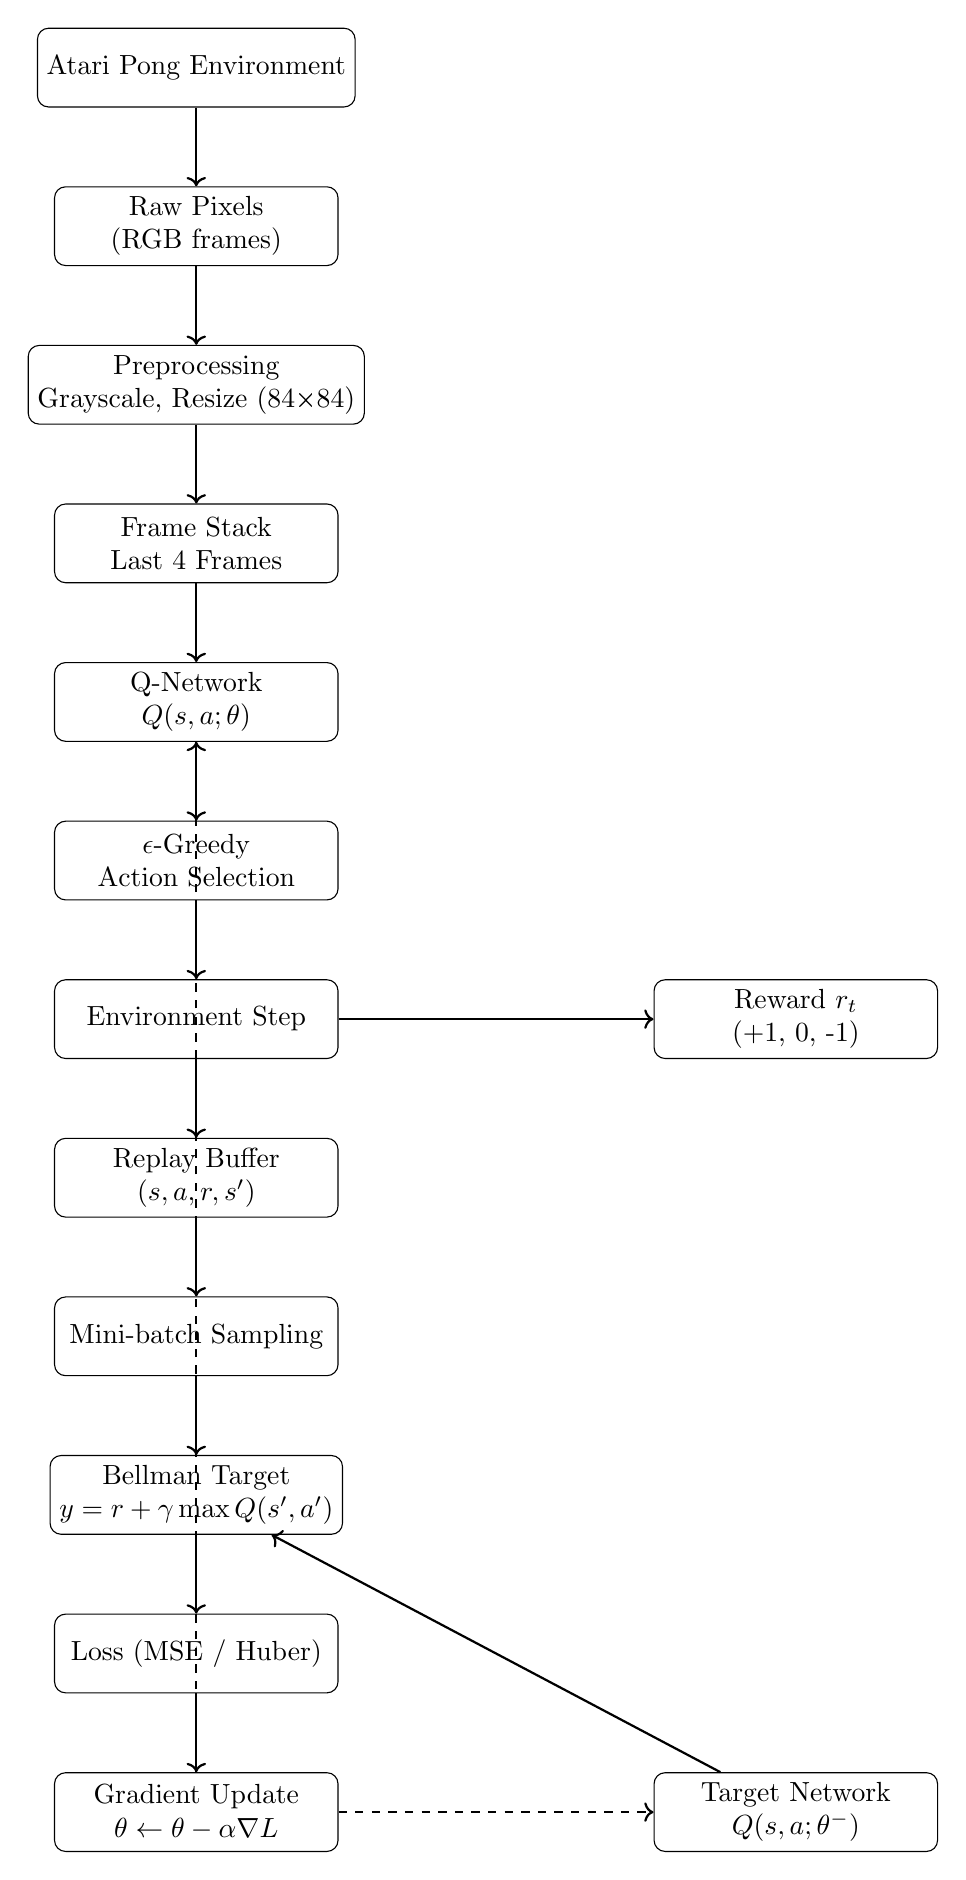
\begin{tikzpicture}[
    box/.style={draw, rectangle, rounded corners, align=center, minimum width=3.6cm, minimum height=1cm},
    arrow/.style={->, thick}
]

% Nodes
\node[box] (env) {Atari Pong Environment};
\node[box, below=of env] (pixels) {Raw Pixels\\(RGB frames)};
\node[box, below=of pixels] (preprocess) {Preprocessing\\Grayscale, Resize (84×84)};
\node[box, below=of preprocess] (stack) {Frame Stack\\Last 4 Frames};
\node[box, below=of stack] (qnet) {Q-Network\\$Q(s,a;\theta)$};
\node[box, below=of qnet] (policy) {$\epsilon$-Greedy\\Action Selection};
\node[box, below=of policy] (step) {Environment Step};
\node[box, right=4cm of step] (reward) {Reward $r_t$\\(+1, 0, -1)};
\node[box, below=of step] (replay) {Replay Buffer\\$(s,a,r,s')$};
\node[box, below=of replay] (sample) {Mini-batch Sampling};
\node[box, below=of sample] (target) {Bellman Target\\$y = r + \gamma \max Q(s',a')$};
\node[box, below=of target] (loss) {Loss (MSE / Huber)};
\node[box, below=of loss] (update) {Gradient Update\\$\theta \leftarrow \theta - \alpha \nabla L$};
\node[box, right=4cm of update] (targetnet) {Target Network\\$Q(s,a;\theta^-)$};

% Arrows
\draw[arrow] (env) -- (pixels);
\draw[arrow] (pixels) -- (preprocess);
\draw[arrow] (preprocess) -- (stack);
\draw[arrow] (stack) -- (qnet);
\draw[arrow] (qnet) -- (policy);
\draw[arrow] (policy) -- (step);
\draw[arrow] (step) -- (replay);
\draw[arrow] (replay) -- (sample);
\draw[arrow] (sample) -- (target);
\draw[arrow] (target) -- (loss);
\draw[arrow] (loss) -- (update);

\draw[arrow] (step) -- (reward);
\draw[arrow] (targetnet) -- (target);
\draw[arrow, dashed] (update) -- (qnet);
\draw[arrow, dashed] (update) -- (targetnet);

\end{tikzpicture}
}
\caption{Deep Q-Network training pipeline for Atari Pong, illustrating the flow from raw pixels to rewards and parameter updates.}
\label{fig:dqn_pong_pipeline}
\end{figure}

\subsection{Appendix B}
This pseudo-code describes the conceptual DQN algorithm implemented in the notebook. Low-level optimisations such as vectorised environments and replay memory internals are abstracted for clarity.

[PLACE HERE ONCE MOST RECENT VERSION IS CONFIRMED]


\end{document}
